%% Short data paper template
%% Created by Simon Hengchen and Nilo Pedrazzini for the Journal of Open Humanities Data (https://openhumanitiesdata.metajnl.com)

\documentclass{article}
\usepackage[spanish]{babel}
\usepackage[utf8]{inputenc}
\usepackage{johd}
\usepackage{booktabs}
\usepackage{tabularx}
\usepackage{graphicx}
\usepackage{hyperref}

\title{\textbf{Predicci\'on de Morosidad}}

\author{Mari\'e del Valle Reyes$^{*}$ \\
        \small $^{*}$\textit{Facultad de Matem\'aticas y Ciencias de la Computaci\'on},\\ \small \textit{Universidad de La Habana, La Habana, Cuba} }

\date{}

\begin{document}
\maketitle


\section{Problema}
Una entidad bancaria está interesada en identificar comportamientos de clientes que puedan derivar en morosidad. Se tiene la información histórica de clientes (\textit{ID}) a
los que les fueron aceptadas sus solicitudes de crédito, conociéndose si el clientes incurrió
(variable \textit{default} = 1) o no (variable \textit{default} = 0) en mora. Las posibles variables de entrada a utilizar para identificar patrones de morosidad son las siguientes:

\begin{itemize}
    \item \textit{Age}: Edad.
    \item \textit{Income}: Ingresos anuales.
    \item \textit{Exp\_Inc}: Proporci\'on del gasto mensual de la tarjeta de cr\'edito para ingresos anuales.
    \item \textit{Avgexp}: Gasto mensual de la tarjeta de cr\'edito.
    \item \textit{Ownrent}: Si es propietario de una vivienda.
    \item \textit{Selfempl}: Si es trabajador por cuenta ajena.
    \item \textit{Depndt}: 1 + N\'umero de dependientes.
    \item \textit{Inc\_per}: Ingresos divididos entre el n\'umero de dependientes.
    \item \textit{Cur\_add}: Meses viviendo en la misma direcci\'on.
    \item \textit{Major}: N\'umero de tarjetas de cr\'edito a cargo.
    \item \textit{Active}: N\'umero de cuentas activas de cr\'edito.
\end{itemize}

Teniendo en cuenta lo anterior, construye un modelo que permita predecir la morosidad de los clientes.

\section{An\'alisis Exploratorio de Datos}

La tabla \ref{tab:addlabel} proporciona un resumen de las variables del problema, incluyendo su tipo, estadísticas descriptivas como mínimo, máximo, media, mediana y desviación típica. 

\begin{table}[h!]
  \centering
  \caption{Resumen de Variables Entradas y Variable Objetivo (default).}
  \begin{tabular}{@{}lcccccc@{}}
    \toprule
    \textbf{Variable} & \textbf{Tipo de variable} & \textbf{Mínimo} & \textbf{Máximo} & \textbf{Media} & \textbf{Mediana} & \textbf{Desviación típica} \\
    \midrule
    Age & numeric & 0.1667 & 83.5 & 33.17 & 30.67 & 10.42 \\
    Income & numeric & 1.5 & 12 & 3.44 & 3 & 1.72 \\
    Exp\_Inc & numeric & 0.0001859 & 0.9063 & 0.09 & 0.061 & 0.11 \\
    Avgexp & numeric & 0 & 2291.17 & 241.76 & 156.09 & 291.09 \\
    Ownrent & integer & 0 & 1 & 0.49 & 0 & 0.50 \\
    Selfempl & integer & 0 & 1 & 0.06 & 0 & 0.24 \\
    Depndt & integer & 0 & 6 & 0.96 & 0 & 1.24 \\
    Inc\_per & numeric & 0.45 & 11 & 2.20 & 2 & 1.33 \\
    Cur\_add & integer & 0 & 540 & 53.99 & 28 & 63.73 \\
    Major & integer & 0 & 1 & 0.84 & 1 & 0.37 \\
    Active & integer & 0 & 29 & 7.35 & 6 & 6.13 \\
    default & integer & 0 & 1 & 0.10 & 0 & 0.31 \\
    \bottomrule
  \end{tabular}%
  \label{tab:addlabel}%
\end{table}%

Las variables Ownrent, Selfempl y default son binarias. La variable objetivo es default, la cual tiene una proporción de 1's de 10.47\%, lo cual significa que aproximadamente el 10.47\% de las observaciones están etiquetadas como clientes que incurren en mora, mientras que el 89.53\% restante están etiquetadas como cliente que no lo hacen. Además, es importante destacar que ninguna de las variables en el conjunto de datos presenta valores faltantes o missings, lo que garantiza la integridad y completitud de los datos para el análisis subsiguiente.

\subsection{Correlaci\'on de las variables}
En la figura \ref{fig:corr_var}, se muestra una matriz de correlaci\'on entre las variables continuas del problema. Las variables cuya correlaci\'on es mayor respecto a las dem\'as son Exp\_Inc y Avgexp con un valor de 0.84. Esto se debe a que ambas variables estan relacionadas con el gasto mensual de la tarjeta de cr\'edito.

\begin{figure}[htbp]
    \centering
    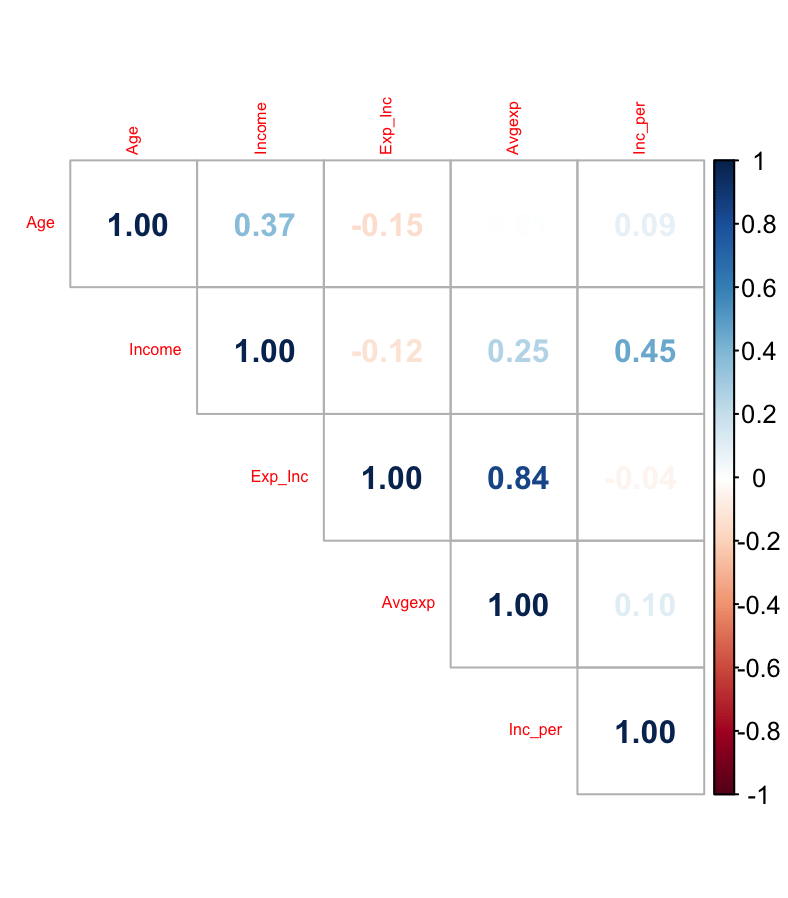
\includegraphics[width=0.5\textwidth]{doc/images/corr.png} 
    \caption{Matriz de correlaci\'on entre variables continuas.}
    \label{fig:corr_var}
\end{figure}

\section{Manipulaci\'on de los datos}

El hecho de que el valor mínimo de la variable Age sea 0.1667 sugiere la presencia de valores atípicos (outliers) en los datos. Estos valores no son consistentes con el contexto del problema. El siguiente gr\'afico (Fig \ref{fig:boxplot_age}) muestra la presencia de valores at\'ipicos en los datos de la variable Age.

\begin{figure}[htbp]
    \centering
    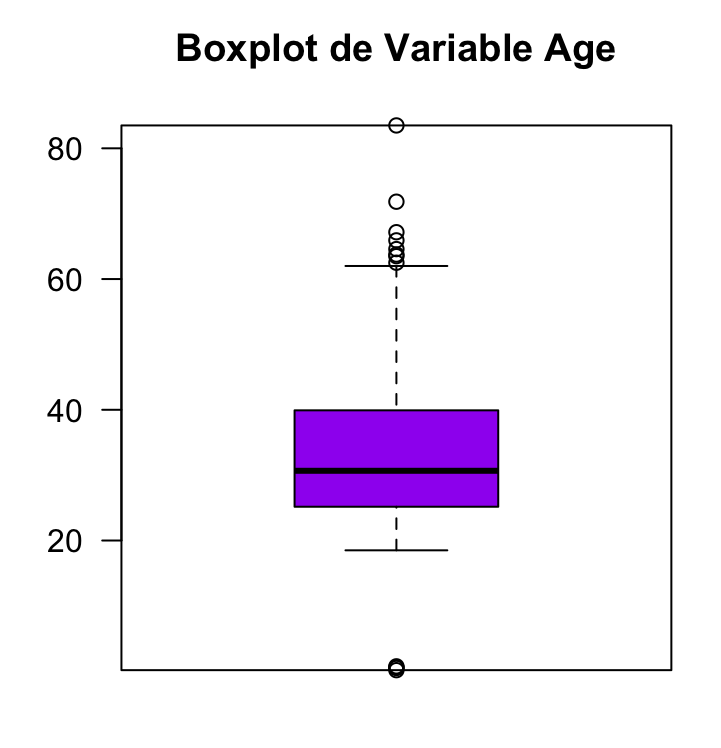
\includegraphics[width=0.5\textwidth]{doc/images/boxplot_age.png} 
    \caption{Boxplot de los datos de la variable Age, en el que se aprecian valores at\'ipicos.}
    \label{fig:boxplot_age}
\end{figure}

Para abordar el problema de los valores atípicos, hay dos enfoques comunes que se pueden considerar. El primero implica eliminar los valores que se encuentran por debajo o por encima de ciertos percentiles de los datos. La Figura \ref{fig:boxplot_age_2} muestra los datos de la variable Age despu\'es de eliminar los datos cuyos cuartiles están por debajo del 0.5\% o por encima del 99.8\%.

\begin{figure}[htbp]
    \centering
    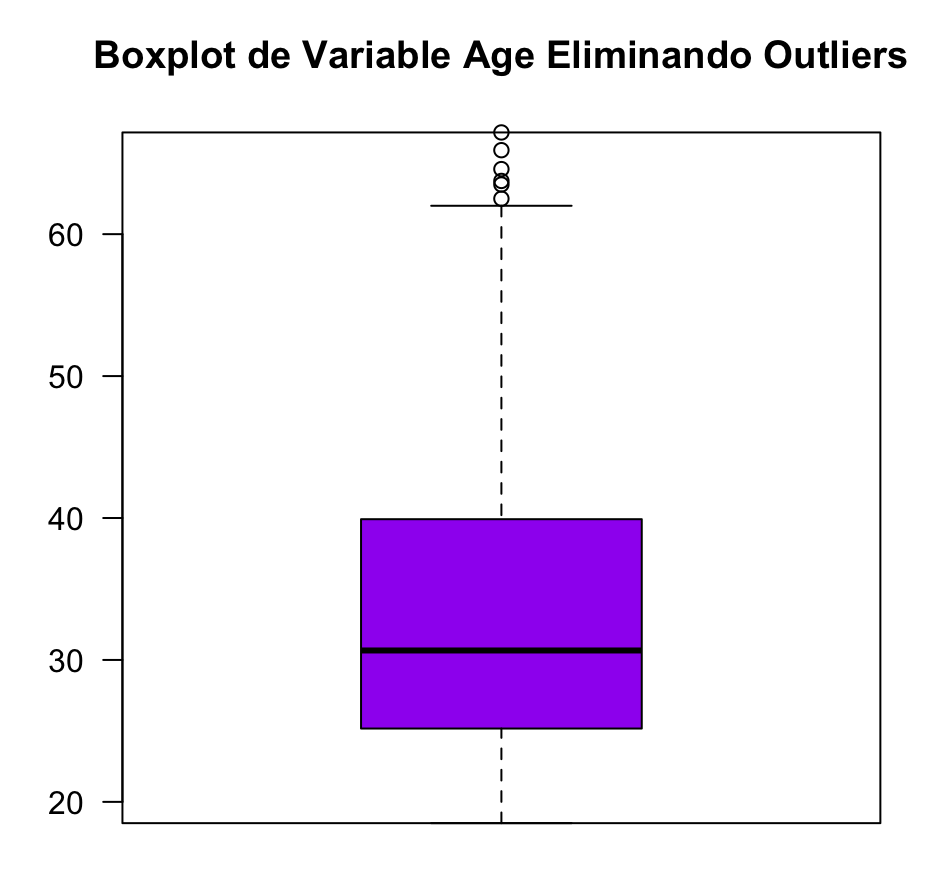
\includegraphics[width=0.5\textwidth]{doc/images/boxplot_age_removing_outliers.png} 
    \caption{Boxplot de los datos de la variable Age. Se eliminaron datos por debajo del percentil 0.05 y por encima del percentil 0.998.}
    \label{fig:boxplot_age_2}
\end{figure}

La segunda opción implica transformar los datos aplicando el logaritmo a la variable. Al aplicar el logaritmo, los valores extremadamente grandes se reducen y los valores extremadamente pequeños se amplifican, lo que puede ayudar a normalizar la distribución de los datos y reducir el impacto de los valores atípicos en el análisis. La siguiente figura (Fig. \ref{hists}) muestra los histogramas de la variable Age antes y despu\'es de aplicar el logaritmo a la variable.

\begin{figure*}[h]
    \centering
    \begin{minipage}[t]{0.45\textwidth}
        \centering
        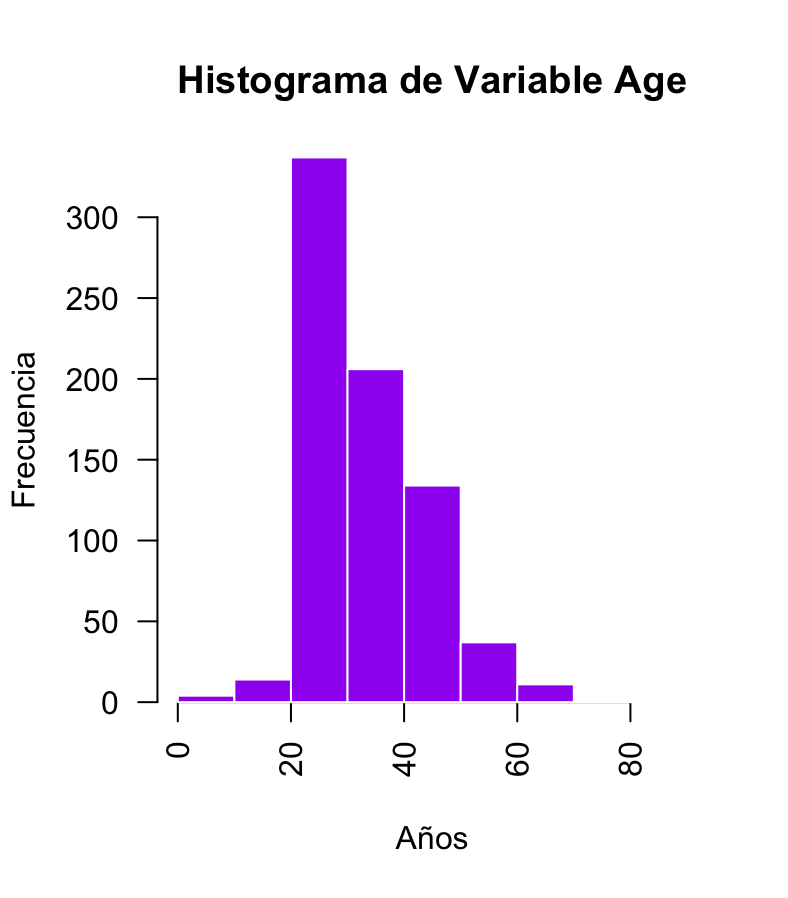
\includegraphics[width=\textwidth]{doc/images/hist_age.png} % Ajusta el ancho de la imagen según tus necesidades
        \caption{Histograma de la variable Age.}
        \label{fig:hist_age}
    \end{minipage}
    \hfill
    \begin{minipage}[t]{0.45\textwidth}
        \centering
        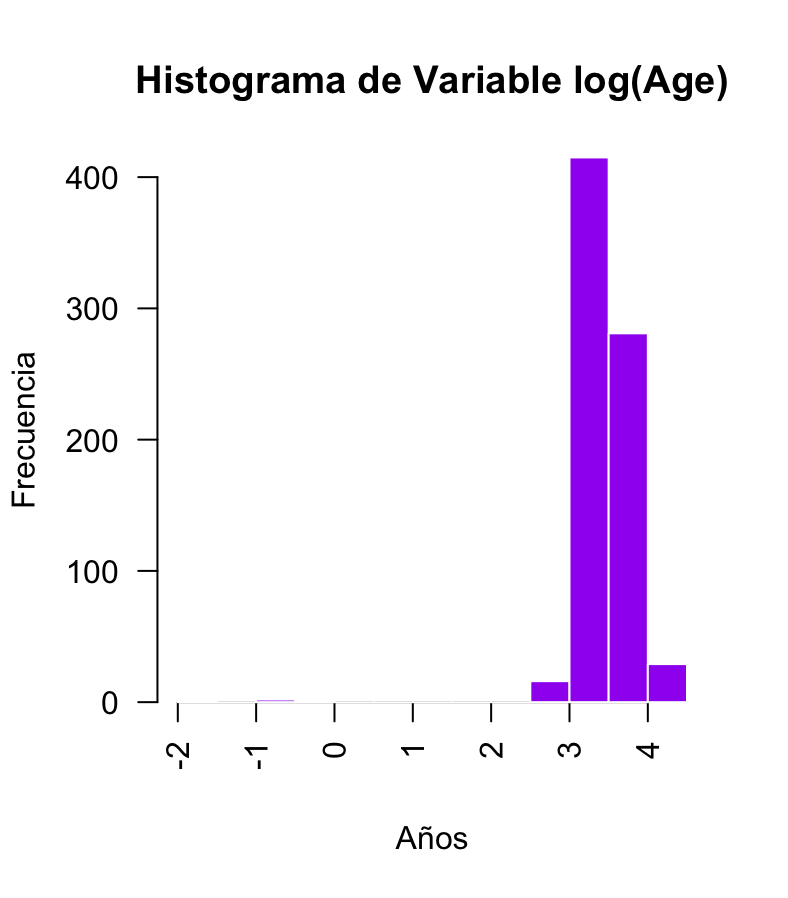
\includegraphics[width=\textwidth]{doc/images/hist_log_age.png} % Ajusta el ancho de la imagen según tus necesidades
        \caption{Histograma de la variable Age despu\'es de aplicarle el logaritmo.}
        \label{fig:hist_age_2}
    \end{minipage}
    \label{hists}
\end{figure*}


\section{Modelo}

En este estudio, se llev\'o a cabo el análisis de un modelos de aprendizaje automático: regresión logística, con el objetivo de predecir la probabilidad de morosidad en un conjunto de datos financiero. Para garantizar la integridad y la calidad de los datos, se utilizó el conjunto de datos de entrenamiento (train), en el cual se eliminaron los valores extremos considerados atípicos. Específicamente, se excluyeron los datos cuyos percentiles eran mayores que el percentil 99.8 y menores que el percentil 0.5. 


\subsection{Regresi\'on log\'istica}

La regresi\'on log\'istica se utiliza para predecir la probabilidad de que ocurra un evento binario en función de una o más variables predictoras.

Primero, se realiz\'o el proceso de selección de variables, en el cual se utiliz\'o el método de pasos. Dicho m\'etodo consiste en encontrar el modelo óptimo que mejor se ajuste a los datos al considerar diferentes combinaciones de variables explicativas. Se comienza con un modelo simple que solo incluye el término de intercepción y se avanza hacia un modelo más complejo que incluye todas las variables disponibles. Todos los modelos intermedios se evalúan y comparan utilizando el criterio de información de Akaike (AIC). Finalmente se selecciona el modelo con el valor de AIC más bajo como el mejor modelo, equilibrando así la precisión predictiva con la complejidad del modelo.

El modelo resultante fue el siguiente:

\begin{equation}
    default = Active + Avgexp + Inc\_per + Cur\_add
\end{equation}


\begin{table}[htbp]
\centering
\begin{tabular}{lcccc}
\hline
Variable & Estimate & Std. Error & Valor z & Pr($>$$|$z$|$) \\
\hline
(Intercept) & -3.7152 & 0.3379 & -10.9936 & $<$ 2.2e-16 \\
Active & 0.0763 & 0.0184 & 4.1483 & 3.35e-05 \\
Avgexp & 0.0010 & 0.0003 & 2.9190 & 0.00351 \\
Inc\_per & 0.1869 & 0.0810 & 2.3064 & 0.0211 \\
Cur\_add & 0.0036 & 0.0016 & 2.2132 & 0.0269 \\
\hline
\end{tabular}
\caption{Estimaciones de los coeficientes de la regresión logística}
\label{tab:regresion-logistica}
\end{table}


En la tabla \ref{tab:regresion-logistica} se observa que los p-valores que indican el nivel de significancia estadística de cada coeficiente, siendo la variable Active la que mayor valor tiene, lo cual prueba su importancia en la predicci\'on de morosidad. Las variables Inc\_per y Cur\_add son moderadamente significativas.

\section{Evaluaci\'on}

Al aplicar el modelo al conjunto de datos test, se contruy\'o una curva ROC (Fig. \ref{fig:roc_regression}) y se calcul\'o el AUC. El valor de AUC es 0.7976889, lo cual indica que el modelo tiene una buena capacidad para clasificar correctamente los casos positivos y negativos en el problema de clasificación binaria.

\begin{figure}[htbp]
    \centering
    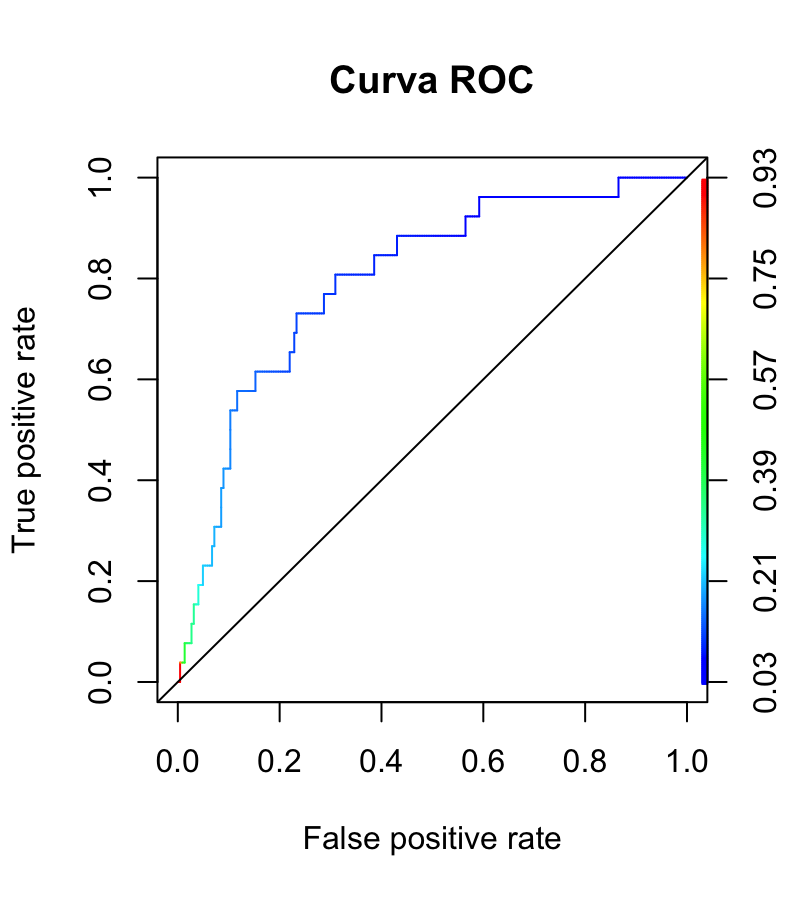
\includegraphics[width=0.5\textwidth]{doc/images/roc_regression.png} 
    \caption{Curva ROC para modelo de regresi\'on log\'istica.}
    \label{fig:roc_regression}
\end{figure}

\section{Repositorio Github}

Los datos, c\'odigo y docuemntaci\'on se encuentran en el repositorio de github \href{https://github.com/marie0501/default-prediction}{default-prediction}.
\end{document}